%%
%% This is file `sample-manuscript.tex',
%% generated with the docstrip utility.
%%
%% The original source files were:
%%
%% samples.dtx  (with options: `manuscript')
%% 
%% IMPORTANT NOTICE:
%% 
%% For the copyright see the source file.
%% 
%% Any modified versions of this file must be renamed
%% with new filenames distinct from sample-manuscript.tex.
%% 
%% For distribution of the original source see the terms
%% for copying and modification in the file samples.dtx.
%% 
%% This generated file may be distributed as long as the
%% original source files, as listed above, are part of the
%% same distribution. (The sources need not necessarily be
%% in the same archive or directory.)
%%
%% Commands for TeXCount
%TC:macro \cite [option:text,text]
%TC:macro \citep [option:text,text]
%TC:macro \citet [option:text,text]
%TC:envir table 0 1
%TC:envir table* 0 1
%TC:envir tabular [ignore] word
%TC:envir displaymath 0 word
%TC:envir math 0 word
%TC:envir comment 0 0
%%
%%
%% The first command in your LaTeX source must be the \documentclass command.
\documentclass[manuscript,screen,review,nonacm]{acmart}
\usepackage{hyperref,xurl}
\usepackage{natbib}
%%
%% \BibTeX command to typeset BibTeX logo in the docs
\AtBeginDocument{%
  \providecommand\BibTeX{{%
    \normalfont B\kern-0.5em{\scshape i\kern-0.25em b}\kern-0.8em\TeX}}}

%% Rights management information.  This information is sent to you
%% when you complete the rights form.  These commands have SAMPLE
%% values in them; it is your responsibility as an author to replace
%% the commands and values with those provided to you when you
%% complete the rights form.
% \setcopyright{acmcopyright}
% \copyrightyear{2018}
% \acmYear{2018}
% \acmDOI{XXXXXXX.XXXXXXX}

%% These commands are for a PROCEEDINGS abstract or paper.
% \acmConference[CS 235]{Data Mining Techniques}{Fall 2023}{University of California, Riverside}
% \acmPrice{15.00}
% \acmISBN{978-1-4503-XXXX-X/18/06}


%%
%% Submission ID.
%% Use this when submitting an article to a sponsored event. You'll
%% receive a unique submission ID from the organizers
%% of the event, and this ID should be used as the parameter to this command.
%%\acmSubmissionID{123-A56-BU3}

%%
%% For managing citations, it is recommended to use bibliography
%% files in BibTeX format.
%%
%% You can then either use BibTeX with the ACM-Reference-Format style,
%% or BibLaTeX with the acmnumeric or acmauthoryear sytles, that include
%% support for advanced citation of software artefact from the
%% biblatex-software package, also separately available on CTAN.
%%
%% Look at the sample-*-biblatex.tex files for templates showcasing
%% the biblatex styles.
%%

%%
%% The majority of ACM publications use numbered citations and
%% references.  The command \citestyle{authoryear} switches to the
%% "author year" style.
%%
%% If you are preparing content for an event
%% sponsored by ACM SIGGRAPH, you must use the "author year" style of
%% citations and references.
%% Uncommenting
%% the next command will enable that style.
%%\citestyle{acmauthoryear}

%%
%% end of the preamble, start of the body of the document source.
\begin{document}

%%
%% The "title" command has an optional parameter,
%% allowing the author to define a "short title" to be used in page headers.
\title{CS235 Fall'23 Project Midterm Report}
%%
%% The "author" command and its associated commands are used to define
%% the authors and their affiliations.
%% Of note is the shared affiliation of the first two authors, and the
%% "authornote" and "authornotemark" commands
%% used to denote shared contribution to the research.
% \author{Ben Trovato}
% \authornote{Both authors contributed equally to this research.}
% \email{trovato@corporation.com}
% \orcid{1234-5678-9012}
% \author{G.K.M. Tobin}
% \authornotemark[1]
% \email{webmaster@marysville-ohio.com}
% \affiliation{%
%   \institution{Institute for Clarity in Documentation}
%   \streetaddress{P.O. Box 1212}
%   \city{Dublin}
%   \state{Ohio}
%   \country{USA}
%   \postcode{43017-6221}
% }

\author{Liam Y. Hsieh (lhsie013)}
\affiliation{
  \institution{University of California, Riverside}
  \streetaddress{900 University Ave}
  \city{Riverside}
  \country{U.S.A}}
\email{liam.hsieh@email.ucr.edu}
\authorsaddresses{}
% \author{Valerie B\'eranger}
% \affiliation{%
%   \institution{Inria Paris-Rocquencourt}
%   \city{Rocquencourt}
%   \country{France}
% }

% \author{Aparna Patel}
% \affiliation{%
%  \institution{Rajiv Gandhi University}
%  \streetaddress{Rono-Hills}
%  \city{Doimukh}
%  \state{Arunachal Pradesh}
%  \country{India}}

% \author{Huifen Chan}
% \affiliation{%
%   \institution{Tsinghua University}
%   \streetaddress{30 Shuangqing Rd}
%   \city{Haidian Qu}
%   \state{Beijing Shi}
%   \country{China}}

% \author{Charles Palmer}
% \affiliation{%
%   \institution{Palmer Research Laboratories}
%   \streetaddress{8600 Datapoint Drive}
%   \city{San Antonio}
%   \state{Texas}
%   \country{USA}
%   \postcode{78229}}
% \email{cpalmer@prl.com}

% \author{John Smith}
% \affiliation{%
%   \institution{The Th{\o}rv{\"a}ld Group}
%   \streetaddress{1 Th{\o}rv{\"a}ld Circle}
%   \city{Hekla}
%   \country{Iceland}}
% \email{jsmith@affiliation.org}

% \author{Julius P. Kumquat}
% \affiliation{%
%   \institution{The Kumquat Consortium}
%   \city{New York}
%   \country{USA}}
% \email{jpkumquat@consortium.net}

%%
%% By default, the full list of authors will be used in the page
%% headers. Often, this list is too long, and will overlap
%% other information printed in the page headers. This command allows
%% the author to define a more concise list
%% of authors' names for this purpose.
%\renewcommand{\shortauthors}{Liam Y. Hsieh}

%%
%% The abstract is a short summary of the work to be presented in the
%% article.
\begin{abstract}
  This midterm report provides an overview of the ongoing CS235 project focused on car sales price prediction. It encompasses the exploration of linear regression as a baseline and delves into the evaluation of 81 distinct Artificial Neural Network (ANN) models. The comparative analysis is based on Mean Absolute Error (MAE) and aims to identify optimal predictive modeling approaches.
\end{abstract}

%%
%% Keywords. The author(s) should pick words that accurately describe
%% the work being presented. Separate the keywords with commas.
\keywords{Car sales price prediction, Neural Networks, Mean Absolute Error (MAE)}


%%
%% This command processes the author and affiliation and title
%% information and builds the first part of the formatted document.
\maketitle

\section{Current State}

The high-level flow for proposed approach is shown as Fig. \ref{fig:flowchart}.   

\begin{figure}
  \centering
  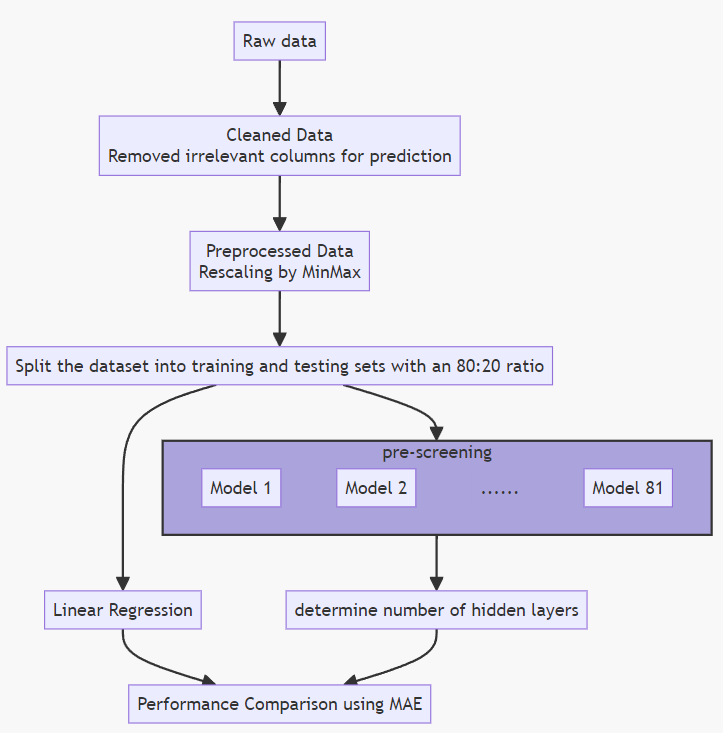
\includegraphics[width=0.8\linewidth]{flowchart.png}
  \caption{Project Overview.}
  \label{fig:flowchart}
\end{figure}

The presented flowchart outlines the sequential steps in a data-driven predictive modeling process. It begins with raw data, progresses through data cleaning and preprocessing, including MinMax normalization. The dataset is then split into training and testing sets with an 80:20 ratio. Two main branches of modeling are pursued: one involves Linear Regression as baseline, and the other explores 81 distinct Artificial Neural Network (ANN) models. The final step involves a comprehensive evaluation of model performance using Mean Absolute Error, providing a comparative analysis between Linear Regression and various ANN models.

\section{Experimental Configuration}
Regarding accurately predicting car sales prices, the existing methods often rely on traditional statistical approaches like linear regression, which has been seen as an acceptable method due to a significant linear relationship being found. The problem at hand involves utilizing Artificial Neural Networks (ANNs), a powerful tool in machine learning, to predict car sales prices to further improve performance. By exploring different ANN architectures and comparing them with a baseline linear regression model, we aim to identify the most effective approach for predicting car sales prices accurately.


\subsection{Linear Regression}
In this predictive modeling task, we aim to utilize linear regression as the baseline method to estimate the car purchase amount based on a set of five input factors. Except for gender which is a binary factor, the other input factors, after MinMax normalization, include the individual's age , annual salary, credit card debt, and net worth, all normalized to fall within the range of 0 to 1.


Linear regression is a statistical method that assumes a linear relationship between the input features and the target variable. In our case, the linear regression model can be expressed as:


\begin{equation*}
y_{\text{price}} = \beta_0 + \beta_1 \cdot X_{\text{gender}} + \beta_2 \cdot X_{\text{age}} + \beta_3 \cdot X_{\text{salary}} + \beta_4 \cdot X_{\text{debt}} + \beta_5 \cdot X_{\text{net\_worth}} + \epsilon
\end{equation*}

where:  
\begin{itemize}
  \item $y_{\text{price}}$ is the predicted car price.
  \item $\beta_0$ is the intercept term.
  \item $\beta_1, \beta_2, \beta_3, \beta_4,\beta_5$ are the coefficients associated with each factor.
  \item $X_{\text{gender}}, X_{\text{age}}, X_{\text{salary}}, X_{\text{debt}}, X_{\text{net\_worth}}$ are input factors.
  \item $\epsilon$ represents the error term, accounting for unobserved factors.
\end{itemize}

The coefficients $\beta_0, \beta_1, \beta_2, \beta_3, \beta_4,\beta_5$ are estimated during the training phase, aiming to minimize the difference between the predicted car price and the actual values in \(y_{\text{price}}\). Once trained, the linear regression model can be used to make predictions on new data, providing insights into the expected car price based on the given input factors.


\subsection{Artificial Neuron Network}

In this project, we systematically investigate the performance of different ANN structures and optimization methods to identify the optimal configuration for predicting our target variable. We consider a range of activation functions, including {\it relu},{\it sigmoid}, and {\it linear} and vary the number of neurons in each layer with choices of 5, 10, and 15 neurons. Additionally, we explore different optimizers, such as {\it adam},{\it sgd}, and {\it nadam}. We generate ANN models based on the combinations of activation functions, neuron counts, and optimizers. All models are compiled using the mean absolute error loss function and mean absolute error as the evaluation metric. For each model we created, we train it on a training set for 100 epochs with a validation split of 20\%. 


\subsubsection{Optimizer}  
\hfill\\
\textbf{Adam (Adaptive Moment Estimation):} Adam maintains two moving averages,$m_t$(mean) and $v_t$(uncentered variance), of the gradients $g_t$. The hyperparameters $\beta_1$ and $\beta_2$ control the decay rates of these moving averages. The $\hat{m}_t$ and $\hat{v}_t$ are bias-corrected estimates. The learning rate $\eta$ is adaptive for each parameter \citep{kingma2014adam}. 

Here is how it update the value:
\begin{align*}
     & m_t = \beta_1 \cdot m_{t-1} + (1 - \beta_1) \cdot g_t \\
     & v_t = \beta_2 \cdot v_{t-1} + (1 - \beta_2) \cdot g_t^2 \\
     & \hat{m}_t = \frac{m_t}{1 - \beta_1^t} \\
     & \hat{v}_t = \frac{v_t}{1 - \beta_2^t} \\
     & \theta_{t+1} = \theta_t - \frac{\eta}{\sqrt{\hat{v}_t} + \epsilon} \cdot \hat{m}_t
\end{align*}

\textbf{Stochastic Gradient Descent (SGD):} As a classic optimization algorithm, it is a computationally efficient option. SGD updates the parameters $\theta$ in the direction of the negative gradient $g_t$ with a fixed learning rate $\eta$.

Here is how SGD update the value:
\begin{equation*}
\theta_{t+1} = \theta_t - \eta \cdot g_t
\end{equation*}

\textbf{Nadam (Nesterov-accelerated Adaptive Moment Estimation):} Nadam incorporates Nesterov momentum into Adam. It combines the advantages of Adam and Nesterov accelerated gradient (NAG) by using the NAG update in the final step \citep{dozat2016incorporating}.

Here is how Nadam update the value:
\begin{align*}
     & m_t = \beta_1 \cdot m_{t-1} + (1 - \beta_1) \cdot g_t \\
     & v_t = \beta_2 \cdot v_{t-1} + (1 - \beta_2) \cdot g_t^2 \\
     & \hat{m}_t = \frac{m_t}{1 - \beta_1^t} \\
     & \hat{v}_t = \frac{v_t}{1 - \beta_2^t} \\
     & \theta_{t+1} = \theta_t - \frac{\eta}{\sqrt{\hat{v}_t} + \epsilon} \cdot (\beta_1 \cdot \hat{m}_t + (1 - \beta_1) \cdot g_t)
\end{align*}

\subsubsection{activation function}
\hfill\\
Here, we briefly summary activation functions existing in this experiment:
\begin{center}
  \begin{tabular}{|l|l|}
    \hline
    \textbf{Activation Function} & \textbf{Mathematical Expression} \\
    \hline
    ReLU (Rectified Linear Unit) & $f(x) = \max(0, x)$ \\
    \hline
    Sigmoid (Logistic Function) & $f(x) = \frac{1}{1 + e^{-x}}$ \\
    \hline
    Linear Activation & $f(x) = x$ \\
    \hline
  \end{tabular}
\end{center}

The experiment aims to analyze and compare the performance of these different configurations, helping us identify the most suitable ANN architecture and optimization strategy for our predictive modeling task.

\section{PRELIMINARY RESULTS}

The code for this project can be found at project repository on GitHub \citep{code}.

All the output results have been illustrated by Fig. \ref{fig:output}. Although linear regression model has relatively low MAE on both training and testing data, we still identify a few ANN models outperforming our baseline. The models with the lowest Test MAE values (indicating better performance on unseen data) are (linear, 5, 15, adam) and (linear, 5, 10, adam), with Test MAE values of 0.000908 and 0.001653, respectively.
Models with {\it adam} as the optimizer generally perform better compared to other optimizers, especially {\it sgd}. Also, models with a linear activation function tend to perform better than other activation functions.
Increasing the number of neurons in the layers does not always result in better performance. Some models with fewer neurons outperform those with more neurons.
The worst-performing models are those using {\it sigmoid} function with {\it sgd} optimizor.

All the output results have been illustrated by Fig. \ref{fig:output}. Although the linear regression model has a relatively low MAE on both training and testing data, we still identify a few ANN models outperforming our baseline. The models with the lowest Test MAE values (indicating better performance on unseen data) are \textbf{(linear, 5, 15, adam)} and \textbf{(linear, 5, 10, adam)}, with Test MAE values of 0.000908 and 0.001653, respectively.
Models with {\it adam} as the optimizer generally perform better compared to other optimizers, especially {\it sgd}. Also, models with a linear activation function tend to perform better than other activation functions.
Increasing the number of neurons in the layers does not always result in better performance. Some models with fewer neurons outperform those with more neurons.
The worst-performing models are those using the {\it sigmoid} function with {\it sgd} optimizer.


\begin{figure}
  \centering
  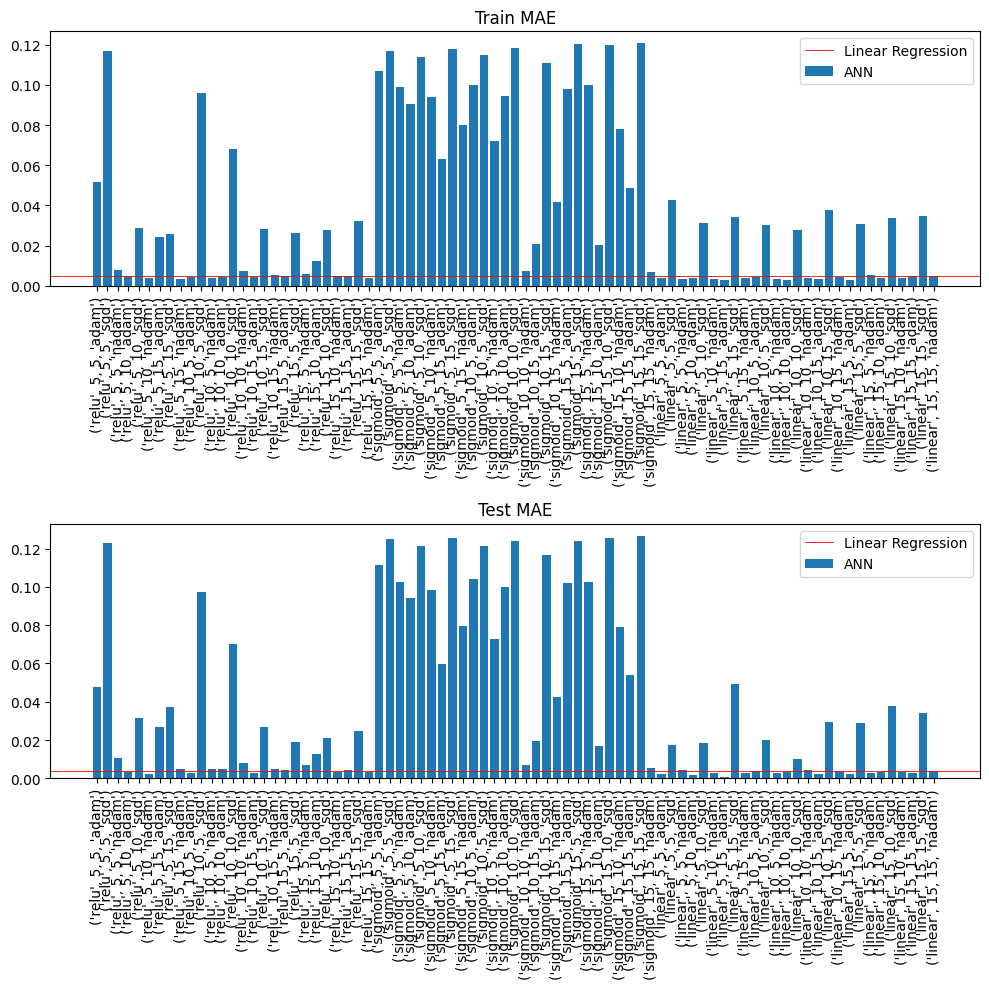
\includegraphics[width=0.8\linewidth]{output.png}
  \caption{Output Overview}
  \label{fig:output}
\end{figure}

We then conduct statistical tests for the best ANN model, \textbf{(linear, 5, 15, adam)},

\begin{table}[h]
  \centering
  \begin{tabular}{|l|l|}
  \hline
  \textbf{Metric} & \textbf{Value} \\
  \hline
  Size of Testing Data & 100 \\
  Variance of Predicted Samples & 0.0239 \\
  Variance of Actual Values & 0.0242 \\
  Standard Deviation of Predicted Samples & 0.1545 \\
  Ratio for Checking Nearly Equal Variance & 0.9867 \\
  T-Statistics & 0.0142 \\
  P Value & 0.9887 \\
  \hline
  \end{tabular}
  \caption{Statistical Test Results}
  \label{tab:statistical_results}
\end{table}
  
Table \ref{tab:statistical_results} summarizes the results of a two-tailed test comparing the variances between the predicted samples and the actual values in the testing dataset. The size of the testing data is 100. The variance of the predicted samples is found to be 0.0239, while the variance of the actual values is 0.0242. The standard deviation of the predicted samples is 0.1545. The ratio for checking nearly equal variance is 0.9867, suggesting a close match between the variances. The calculated t-statistics is 0.0142, and the associated p-value is 0.9887. With a p-value greater than the commonly used significance level of 0.05, we do not have sufficient evidence to reject the null hypothesis. Therefore, we conclude that there is no significant difference in variances between the predicted samples and the actual values; the prediction model we proposed can perform a satisfactory output.
\bibliographystyle{ACM-Reference-Format}
\bibliography{reference}
\end{document}
\endinput
%%
%% End of file `sample-manuscript.tex'.
